\documentclass[tikz]{standalone}
\input{../tikz/plots_config.pgs}

\begin{document}

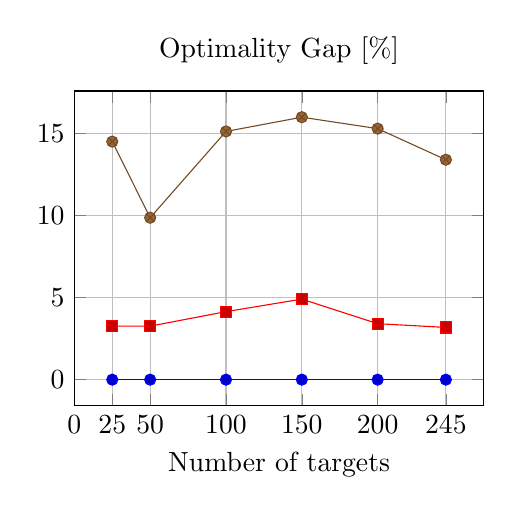
\begin{tikzpicture}
\begin{axis}[%
width=52mm,
height=40mm,
scale only axis,
xmin=0,
xmax=270,
xtick={ 0,  25,  50, 100, 150, 200, 245},
xmajorgrids,
ymajorgrids,
title={Optimality Gap [\%]},
xlabel={Number of targets},
]
% Exact
\addplot coordinates{
  (25,0.00000)
  (50,0.00000)
  (100,0.00000)
  (150,0.00000)
  (200,0.00000)
  (245,0.00000)
};

% 2-Opt
\addplot coordinates{
  (25,3.25970)
  (50,3.25970)
  (100,4.14214)
  (150,4.90516)
  (200,3.40849)
  (245,3.18091)
};

% RNN
\addplot coordinates{
  (25,14.49900)
  (50,9.86297)
  (100,15.11878)
  (150,15.98574)
  (200,15.28930)
  (245,13.39406)
};
\end{axis}
\end{tikzpicture}

\end{document}
